\section{Data Generation Taxonomy}\label{sec:taxonomy}

The taxonomy proposed in this paper is a combination of
different definitions found in the literature, extended with other traits that
vary among domains and generation techniques. Within image data studies,
\cite{shorten2019survey} and \cite{khalifa2021comprehensive} divide data
augmentation techniques into ``basic'' or ``classical'' approaches and deep
learning approaches. In both cases, the former refers to domain-specific
generation techniques, while the latter may be applied to any data structure.
\cite{iwana2021empirical} proposes a time-series data augmentation taxonomy
divided into four families: (1) Random transformation, (2) Pattern mixing, (3)
Generative models, and (4) Decomposition. Except for generative models,
the majority of the methods presented in the remaining families are
well-established and domain-specific. \cite{hernandez2022synthetic}
defines a taxonomy for synthetic tabular data generation approaches divided
into three types of approaches: (1) Classical, (2) Deep learning, and (3)
Others. Most taxonomies follow similar definitions while varying in
terminology or distinction criteria. In addition, all taxonomies with
categories defined as ``basic'', ``traditional'', or ``classical'' use these to
characterize domain-specific transformations.

Within the taxonomies found, none of them consider how a generation
mechanism employs $\mathcal{D}$ into the generation process or, if
applicable, the training phase. However, it is important to understand whether
a generation mechanism randomly selects $x$ and a set of close neighbors, thus
considering local information only, or considers the overall dataset or data
distribution for the selection of $x$ and/or generation of $x^s$. Our
proposed taxonomy is depicted in Figure~\ref{fig:data-generation-taxonomy}. It
characterizes data generation mechanisms using four properties:

\begin{enumerate}

    \item Architecture. Defines the broader type of data augmentation. It is
        based on domain specificity, architecture type, or data transformations
        using a heuristic or random perturbation process. Data generation
        based on data sampling from a probability function is considered
        probability-based. Generation techniques that apply a form of random
        perturbation, interpolation, or geometric transformation to the data
        with some degree of randomness are considered randomized approaches.
        Typical, domain-specific data generation techniques are considered
        domain-specific approaches. These techniques apply transformations to
        a data point leveraging relationships in the structure of the data
        (which is known \textit{a priori}). Generative models based on neural
        network architectures are defined as network-based. These
        architectures attempt to either generate observations in the latent
        space and/or by producing observations that are difficult to
        distinguish from the original dataset.

    \item Application level. Refers to the phase of the ML pipeline where the
        generative process is included. Generative models are considered
        internal if used alongside the primary ML task, whereas
        models used before the development of the primary ML task are
        considered external.

    \item Scope. Considers the usage of the original dataset's properties.
        Generative models that consider the density of the data space,
        statistical properties of $\mathcal{D}$, or attempt to
        replicate/manipulate specific relationships found in $\mathcal{D}$ are
        considered to have a global scope, whereas generative models that
        consider a single observation and/or a set of close neighbors are
        considered to have a local scope. On the one hand, generative models
        with a local scope do not account for $\mathbb{P}^s$ but allow for the
        generation of $x^s$ within more precise regions in the
        latent/input space. On the other hand, generative models with a
        global scope have a higher capacity to model $\mathbb{P}^s$ but
        produce $x^s$ with less precision within the latent/input
        space.

    \item Data space. Refers to the type of data representation used to apply
        the generative model. Generation mechanisms can be applied using the
        raw dataset (\textit{i.e.}, on the input space), an embedded
        representation of the data (\textit{i.e.}, on the latent space), or
        based on the target feature (\textit{i.e.}, on the output space).
        Although some studies discuss the need to generate synthetic data on
        the input space~\cite{dankar2021fake, patki2016synthetic}, 
        various studies successfully apply synthetic data generation
        techniques on a latent space.

\end{enumerate}

\begin{figure}
	\centering
	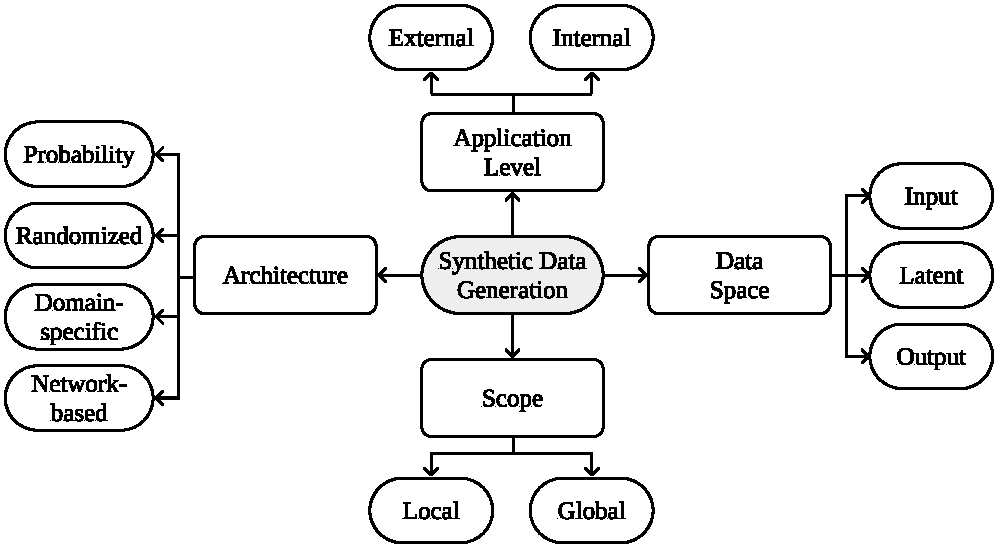
\includegraphics[width=.95\linewidth]{../analysis/data-generation-taxonomy}
    \caption{General taxonomy of data generation mechanisms proposed in this
        paper.
    }~\label{fig:data-generation-taxonomy}
\end{figure}

Throughout the analysis of the different types of generation mechanisms, all
relevant methods were characterized using this taxonomy and listed in
Table~\ref{tbl:generators}.

\begingroup\small
\setlength\LTleft{-1.5cm}
\setlength\LTright{1.5cm}
\begin{longtable}{rcccccccc}
    \caption{Summary of the synthetic data generation methods discussed in
    this work. A field containing ``---'' indicates that the it is either
    not applicable to the corresponding method, and/or applies its own unique
    approach.}
    \label{tbl:generators}\\
    \toprule
               Algorithm & ML Problem & Type &  Architecture & Level &  Data
               Space & Scope \\
    \midrule
    \endfirsthead
    \caption[]{Summary of the synthetic data generation methods discussed in
    this work. A field containing ``---'' indicates that the it is either
    not applicable to the corresponding method, and/or applies its own unique
    approach.} \\
    \toprule
               Algorithm & ML Problem & Type &  Architecture & Level &  Data
               Space & Scope \\
    \midrule
    \endhead
    \midrule
    \multicolumn{9}{r}{{Continued on next page}} \\
    \midrule
    \endfoot
    
    \bottomrule
    \endlastfoot
    SDV~\cite{patki2016synthetic} & Anon. & PDF & Probabilistic & External & Input & Global \\
    MST~\cite{mckenna2021winning} & DP & PGM & Probabilistic & External & Input & Global \\
    MWEM~\cite{hardt2012simple} & DP & Other & Probabilistic & External & Input & Global \\
    MWEM-PGM~\cite{mckenna2019graphical} & DP & PGM & Probabilistic & External & Input & Global \\
    PrivBayes~\cite{zhang2017privbayes} & DP & PGM & Probabilistic & External & Input & Global \\
    DPGAN~\cite{xie2018differentially} & DP & GAN & Network & External & Latent & Global \\
    DPCTGAN~\cite{rosenblatt2020differentially} & DP & GAN &  Network & External & Latent & Global \\
    PATE-GAN~\cite{jordon2018pate} & DP & GAN & Network & External & Lat. + Out. & Global \\
    PATECTGAN~\cite{rosenblatt2020differentially} & DP & GAN & Network & External & Lat. + Out. & Global \\
    FEM~\cite{vietri2020new} & DP & Perturb. & Probabilistic & External & Input & Global \\
    RAP~\cite{aydore2021differentially} & DP & Perturb. & Probabilistic & External & Input & Global \\
    PDF~\cite{de2019formal, suciu2011probabilistic} & --- & PDF & Probabilistic & External & Input & Global \\
    Kamino~\cite{ge2021kamino} & DP & PDF & Probabilistic & External & Input & Global \\
    RON-GAUSS~\cite{chanyaswad2019ron} & DP & PDF & Probabilistic & Internal & Latent & Global \\
    HDMM~\cite{mckenna2018optimizing} & DP & Perturb. & Probabilistic & External & Input & Global \\
    DualQuery~\cite{gaboardi2014dual} & DP & Other & Probabilistic & External & Input & Global \\
    ROS(E)~\cite{menardi2014training} & Ovs & Perturb. & Randomized & External & Input & Local \\ 
    SMOTE~\cite{chawla2002smote} & Ovs & Linear & Randomized & External & Input & Local \\
    SMOTENC~\cite{chawla2002smote} & Ovs & Linear & Randomized & External & Input & Local \\
    SMOTEN~\cite{chawla2002smote} & Ovs & --- & --- & External & Input & Local \\
    Borderline-SMOTE~\cite{han2005borderline} & Ovs & Linear & Randomized & External & Input & Local \\
    G-SMOTE~\cite{douzas2019geometric} & Ovs & Geometric & Randomized & External & Input & Local \\
    ADASYN~\cite{he2008adasyn} & Ovs & Linear & Randomized & External & Input & Local \\
    KernelADASYN~\cite{tang2015kerneladasyn} & Ovs & PDF & Probabilistic & External & Input & Local \\
    MOKAS~\cite{lin2017minority} & Ovs & Other & Network & External & Latent & Global \\
    SOMO~\cite{douzas2017self} & Ovs & Linear & Net.+Rand. & External & Input & Global \\
    G-SOMO~\cite{douzas2021g} & Ovs & Geometric & Net.+Rand. & External & Input & Global \\
    GMM-SENN~\cite{xing2022predict} & Ovs & PDF & Probabilistic & External & Input & Global \\
    GMF-SMOTE~\cite{xu2022synthetic} & Ovs & Linear & Randomized & External & Input & Global \\
    C-VAE~\cite{dai2019generative} & Ovs & AE & Network & External & Latent & Global \\
    Safe-level SMOTE~\cite{bunkhumpornpat2009safe} & Ovs & Linear & Randomized & External & Input & Local \\
    LR-SMOTE~\cite{liang2020lr} & Ovs & Linear & Randomized & External & Input & Global \\
    K-means SMOTE~\cite{douzas2018improving} & Ovs & Linear & Randomized & External & Input & Global\\
    DBSMOTE~\cite{bunkhumpornpat2012dbsmote} & Ovs & Linear & Randomized & External & Input & Local\\
    CGAN~\cite{douzas2018effective} & Ovs & GAN & Network & External & Latent & Global \\
    K-means CTGAN~\cite{an2021k} & Ovs & GAN & Network & External & Latent & Global \\
    SMOTER~\cite{torgo2013smote} & Ovs + Reg & Linear & Randomized & External & Input & Local \\
    G-SMOTER~\cite{camacho2022geometric} & Ovs + Reg & Linear & Randomized & External & Input & Local \\
    RACOG~\cite{das2014racog} & Ovs & PGM & Probabilistic & External & Input & Global \\
    wRACOG~\cite{das2014racog} & Ovs & PGM & Probabilistic & External & Input & Global \\
    RWO~\cite{zhang2014rwo} & Ovs & PGM & Probabilistic & External & Input & Global \\
    PDFOS~\cite{gao2014pdfos} & Ovs & PDF & Probabilistic & External & Input & Global \\
    Mixup~\cite{zhang2018mixup} & DA & Linear & Randomized & External & In.+Out. & Local \\
    M-Mixup~\cite{verma2019manifold} & DA & Linear & Network & Internal & Lat.+Out. & Global \\
    NL-Mixup~\cite{guo2020nonlinear} & DA & Geometric & Randomized & External & In.+Out. & Local \\
    AE-DA~\cite{feng2020autuencoder} & DA & AE & Network & External & In./Lat.+Out. & Local \\
    MODALS~\cite{cheung2020modals} & DA & --- & Network & Internal & Latent & Global \\
    LSI~\cite{liu2018data} & DA & AE & Network & External & Lat.+Out. & Global \\
    Gibbs~\cite{fakoor2020fast} & DA & PGM & Probabilistic & External & Input & Global \\
    MedGAN~\cite{armanious2020medgan} & DA & GAN & Network & External & Latent & Global \\
    GANBLR~\cite{zhang2021ganblr} & DA & PGM & Probabilistic & External & Input & Global \\
    Table-GAN~\cite{park2018data} & DA & GAN & Network & External & Latent & Global \\
    CTGAN~\cite{xu2019modeling} & DA & GAN & Network & External & Latent & Global \\
    TVAE~\cite{xu2019modeling} & DA & AE & Network & External & Latent & Global \\
    AE~\cite{delgado2021deep} & DA & AE & Network & External & Latent & Global \\
    InfoMixup~\cite{kim2021lada} & AL & Linear & Network & Internal & Lat.+Out. & Global \\
    VAEACGAN~\cite{tran2019bayesian} & AL & AE & Network & Internal & Latent & Global\\
    AL-G-SMOTE~\cite{fonseca2021increasing} & AL & Geometric & Randomized & Internal & Input & Local\\
    DAE~\cite{rasmus2015semi} & Semi-SL & AE & Network & Internal & Input & Global \\ 
    $\Pi$-model~\cite{samuli2017temporal} & Semi-SL & Perturb. & Randomized & Internal & In.+Lat. & Local \\
    Mean Teacher~\cite{tarvainen2017mean} & Semi-SL & Perturb. & Randomized & Internal & In.+Lat. & Local \\
    ICT~\cite{verma2022interpolation} & Semi-SL & Linear & Randomized & Internal & Input & Local \\
    Mixmatch~\cite{berthelot2019mixmatch} & Semi-SL & Linear & Randomized & Internal & Input & Local \\
    SDAT~\cite{fang2022semi} & Semi-SL & AE+PDF & Net.+Prob. & Internal & Latent & Global \\
    MCoM~\cite{li2022mcom} & Semi-SL & Linear & Randomized & Int.+Ext. & Inp.+Lat. & Global \\
    C-Mixup~\cite{darabi2021contrastive} & Semi/Self-SL & AE+Lin. & Net+Rand.  & Internal & Latent & Global \\
    VIME~\cite{yoon2020vime} & Semi/Self-SL & Perturb. & Randomized & Internal & Input & Local \\
    SubTab~\cite{ucar2021subtab} & Self-SL & Perturb. & Rand.+Prob. & Internal & Input & Local \\
    Scarf~\cite{bahri2022scarf} & Self-SL & Perturb. & Randomized & Internal & Input & Local \\
    A-SFS~\cite{qiu2022sfs} & Self-SL & Perturb. & Randomized & Internal & Input & Local \\
\end{longtable}
\endgroup

